\section*{3 Random Projections}

\subsection*{Problem 7}

Consider the 1D situation. Then there are only two possible cases:

\begin{itemize}
  \item the vectors $\mathbf{u}$ and $\mathbf{v}$ are parallel\\
Then $h_r(\mathbf{u}) = h_r(\mathbf{v})$ is always fulfiled and 
\[p(h_r(\mathbf{u}) = h_r(\mathbf{v})) = 1-\frac{0}{\pi} = 1\]
  \item the vectors $\mathbf{u}$ and $\mathbf{v}$ are antiparallel\\
Then $h_r(\mathbf{u}) = - h_r(\mathbf{v})$ and 
\[p(h_r(\mathbf{u}) = h_r(\mathbf{v})) = 1-\frac{\pi}{\pi} = 0\]
\end{itemize}

Now suppose we are in 2D. It is sufficient to show that \[p\left(h_r(\mathbf{u}) \neq h_r(\mathbf{v})\right)=\frac{\theta(\mathbf{u}, \mathbf{v})}{\pi}.\] Then \[p\left(h_r(\mathbf{u}) = h_r(\mathbf{v})\right) = 1-p\left(h_r(\mathbf{u}) \neq h_r(\mathbf{v})\right) = 1 - \frac{\theta(\mathbf{u}, \mathbf{v})}{\pi}.\]

Let $u_\perp$, $v_\perp$ be the lines, perpendicular to $\mathbf{u}$ and $\mathbf{v}$, respectively. Then the probability that $h_r(\mathbf{u})$ is not equal to $h_r(\mathbf{v})$ is the same as the probability of choosing any point in the plane, which falls in the shaded region in Fig. \ref{fig:theta}. From simple geometry, the angle between $\mathbf{u_\perp}$ and $\mathbf{v_\perp}$ is equal to $\theta(\mathbf{u,v})$. Thus the probability that a randomly chosen point in the plane falls in the shaded region is equal to $\frac{2\theta}{2\pi}=\frac{\theta}{\pi}$, which we wanted to show.
\begin{figure}[!h]
  \begin{center}
    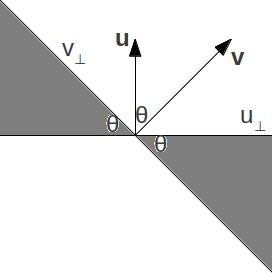
\includegraphics[width=0.25\textwidth]{plots/3.png}
    \caption{2D diagram}
    \label{fig:theta}
  \end{center}
\end{figure}

Now suppose that we are in a higher dimensional space. Then if $\mathbf{u}$ and $\mathbf{v}$ are not parallel or antiparallel (in which case we come down to the same calculation as in 1D, which we already showed), they define a unique plane that contains both of them. It is sufficient to consider the projection of $\mathbf{r}$ onto that plane and whether it lies in the same shaded region as in 2D, hence the problem is reduced to the 2D case.

